\documentclass{article}
\usepackage{main}

\title{Exercices : résolution graphique d'équations et d'inéquations}
\author{Seconde 9}
\date{10 Mars 2025}

\begin{document}
\maketitle

\begin{minipage}{0.45\textwidth}
\begin{center}
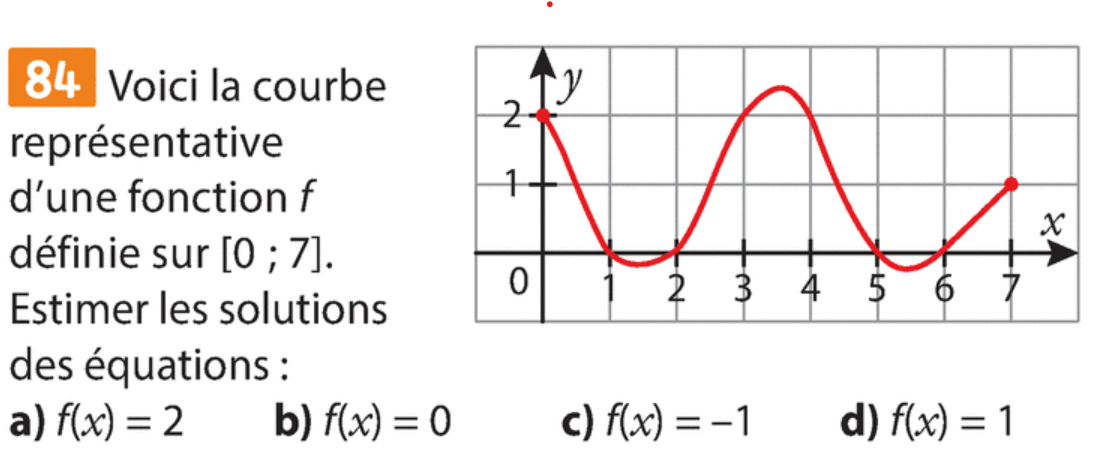
\includegraphics[width=\textwidth]{Exercice_1.png}
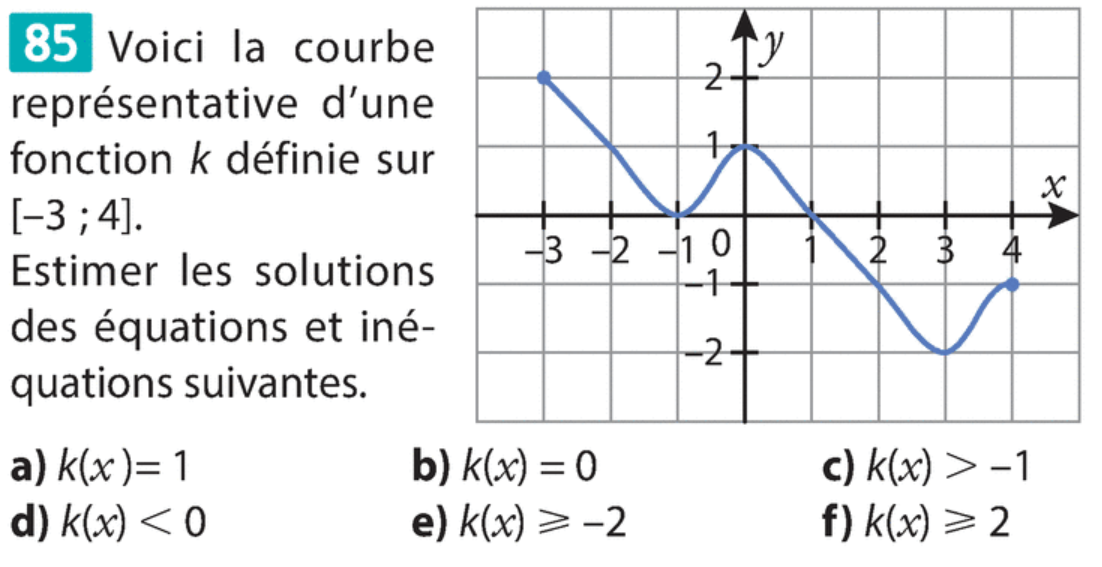
\includegraphics[width=\textwidth]{Exercice_2.png}
\end{center}    
\end{minipage}
\hfill\vline\hfill
\begin{minipage}{0.45\textwidth}
\begin{center}
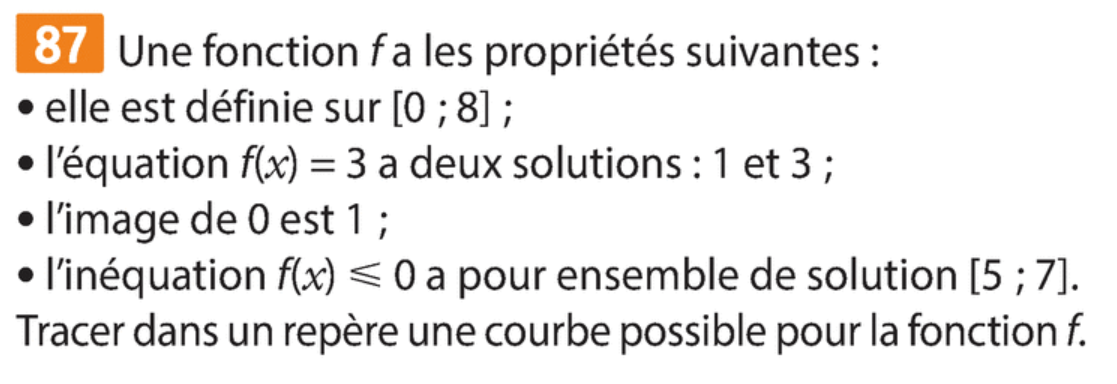
\includegraphics[width=\textwidth]{Exercice_3.png}
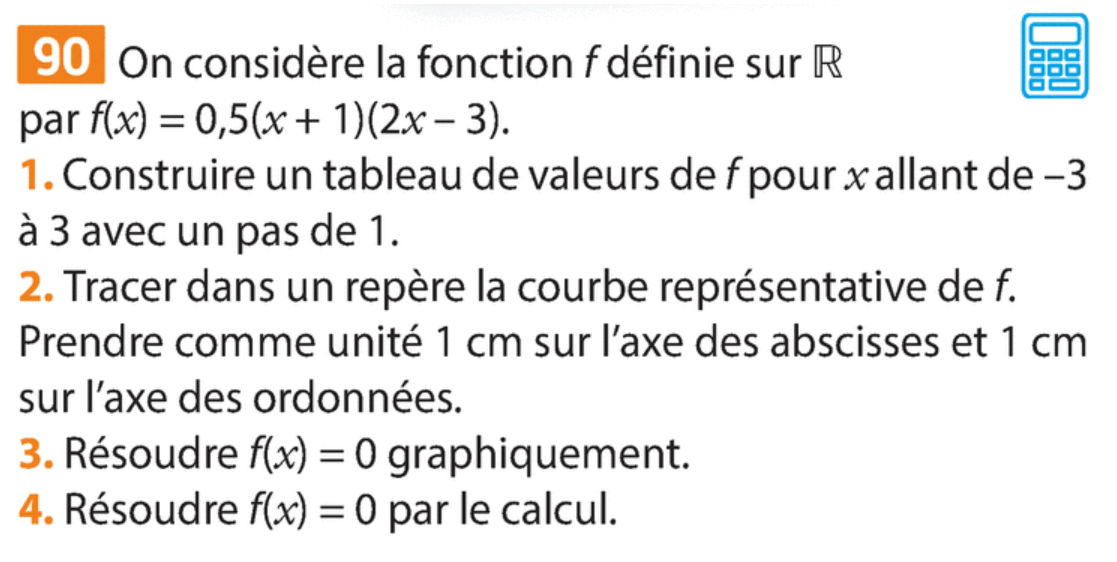
\includegraphics[width=\textwidth]{Exercice_4.png}
\end{center}
\end{minipage}
\vspace*{0.5cm}
\begin{minipage}{0.45\textwidth}
\begin{center}
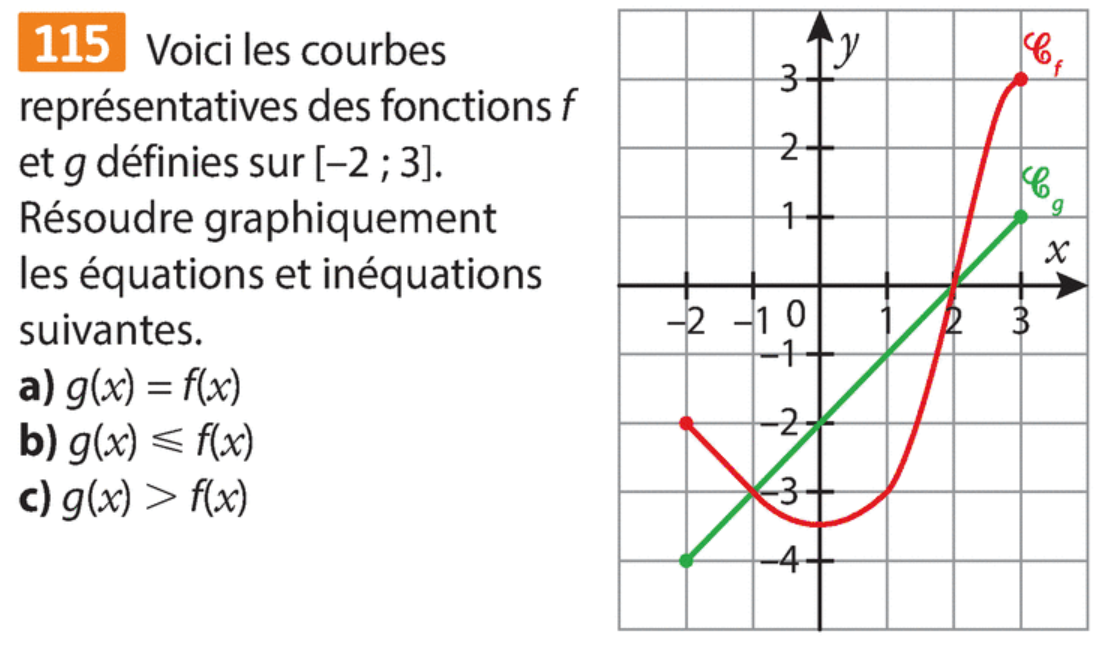
\includegraphics[width=\textwidth]{Exercice_5.png}
\end{center}    
\end{minipage}
\hfill\vline\hfill
\begin{minipage}{0.45\textwidth}
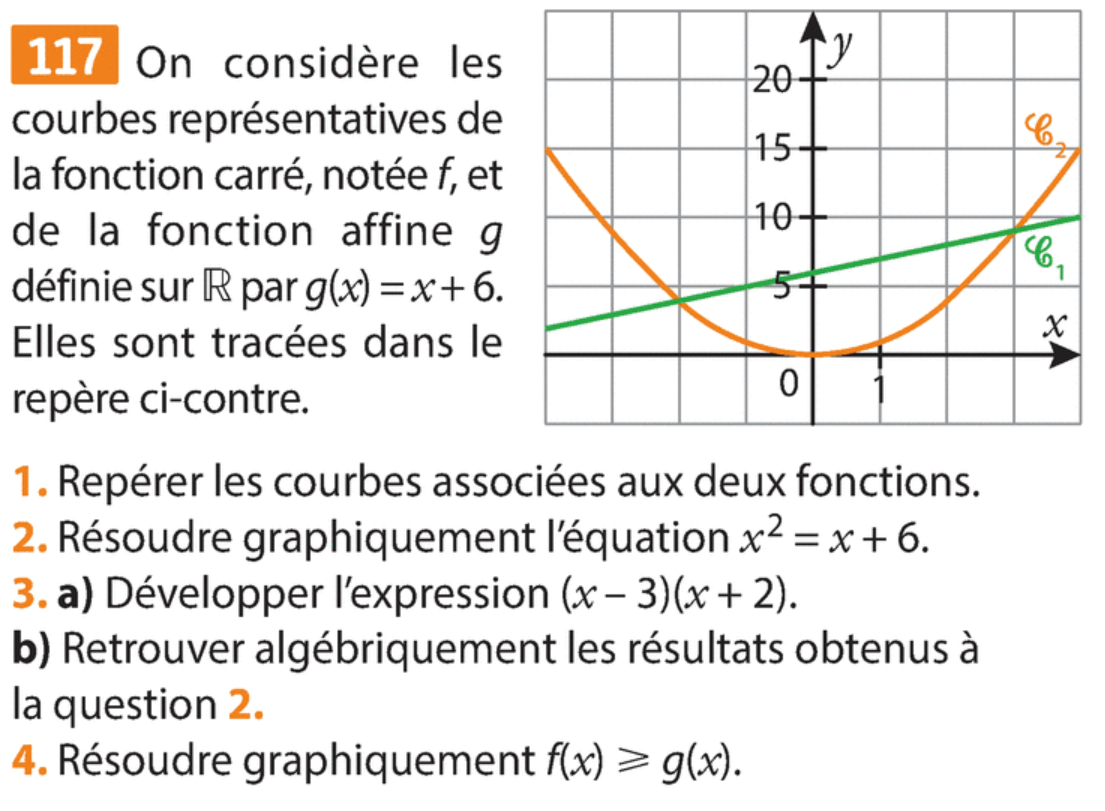
\includegraphics[width=\textwidth]{Exercice_6.png}
\end{minipage}
\begin{center}
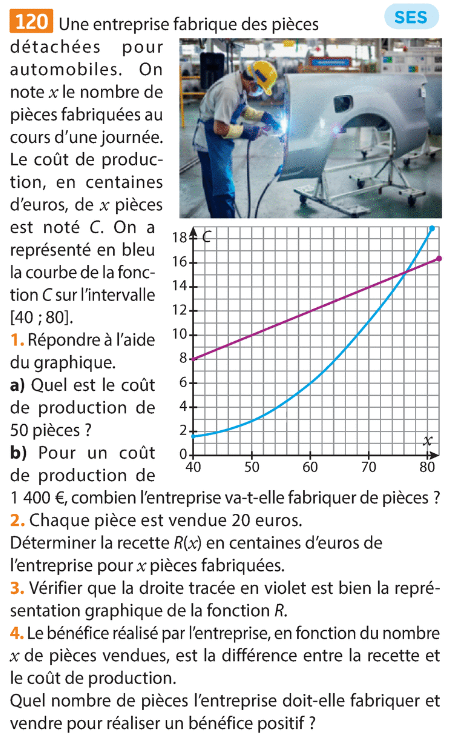
\includegraphics[width=\textwidth]{Exercice_7.png}
\end{center}
\end{document}